\documentclass[12pt,a4paper]{report}
\usepackage[utf8]{inputenc}
\usepackage{graphicx}
\usepackage{float}
\usepackage{booktabs}
\usepackage{hyperref}
\usepackage{tikz}
\usetikzlibrary{shapes.geometric, arrows, positioning, calc, backgrounds, fit}
\usepackage{geometry}
\geometry{a4paper, margin=1in}

\title{
    \vspace{2cm}
    \textbf{\Huge Multi-Vital Health Monitor Project Report}\\
    \vspace{1cm}
    \large \textbf{An ESP32-based Real-time Wearable Health Monitor}\\
    \vspace{2cm}
}
\author{Developed by the Engineering Team}
\date{\today}

\begin{document}

\maketitle

\begin{abstract}
This comprehensive report outlines the design, development, and implementation of a real-time, wearable Multi-Vital Health Monitor. Built on the dual-core ESP32 microcontroller and utilizing the FreeRTOS real-time operating system, this device seamlessly acquires and processes multiple health metrics concurrently. The integration includes heart rate and SpO2 tracking (MAX30102), clinical-grade body temperature monitoring (MAX30205), and fall detection (MPU6050). The report delves into the intricate details of hardware wiring, power regulation architectures (including TP4056, 5V step-up modules, and AMS1117), task logical flows, and the rationale behind specific RTOS configuration parameters.
\end{abstract}

\tableofcontents
\newpage

\chapter{Introduction}
The demand for continuous, non-invasive health monitoring in wearable formats has grown exponentially. The Multi-Vital Health Monitor bridges the gap between commercial off-the-shelf medical devices and open-source hobbyist electronics. By leveraging the ESP32's dual-core architecture and FreeRTOS, the device achieves deterministic real-time data acquisition without compromising network throughput or user interface responsiveness. This project places heavy emphasis on robust power management, precise task scheduling, and stable I2C bus arbitration.

\chapter{Project Context}
The system operates within a broader ecosystem connecting the end-user (patient) to medical monitoring dashboards.
\section{System Context Diagram}

\begin{figure}[H]
    \centering
    \resizebox{\textwidth}{!}{
    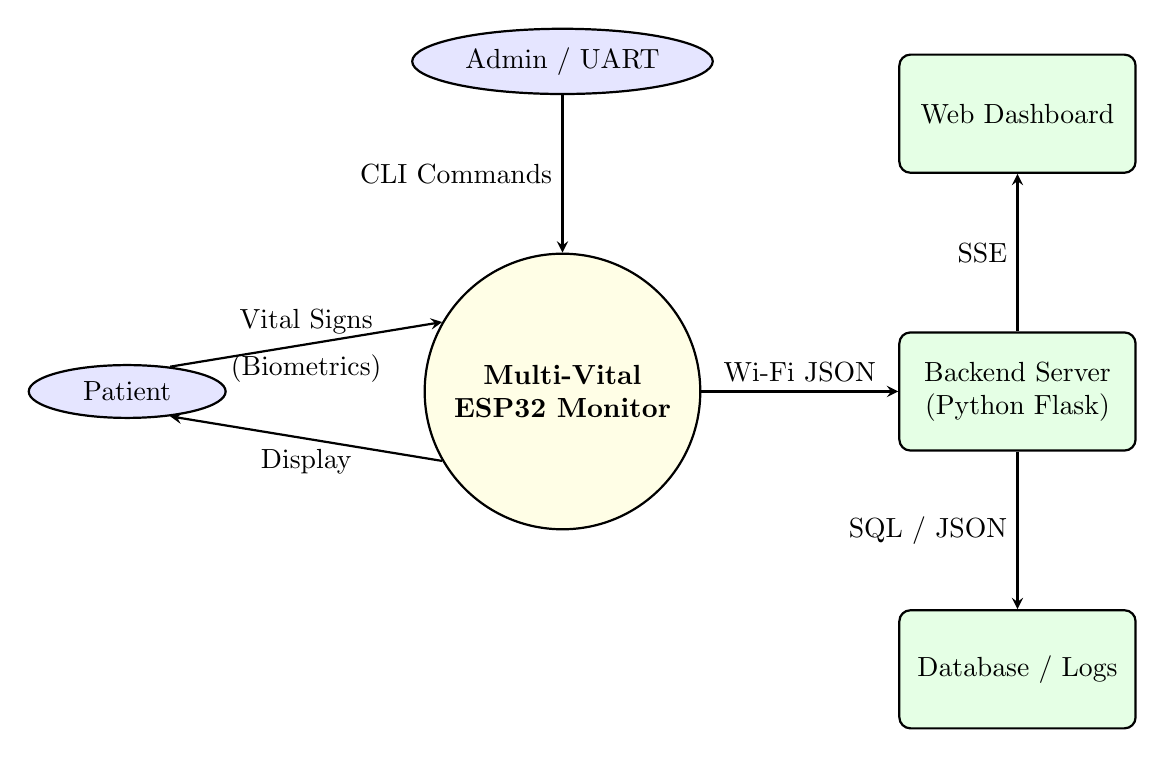
\begin{tikzpicture}[
        node distance=2cm and 2.5cm,
        actor/.style={ellipse, draw=black, fill=blue!10, minimum width=2.5cm, align=center, thick},
        system/.style={circle, draw=black, fill=yellow!10, minimum size=3.5cm, align=center, thick},
        external/.style={rectangle, draw=black, fill=green!10, rounded corners, minimum width=3cm, minimum height=1.5cm, align=center, thick},
        arrow/.style={thick,->,>=stealth}
    ]
        % Nodes
        \node[system] (esp32) {\textbf{Multi-Vital}\\\textbf{ESP32 Monitor}};
        \node[actor, left=of esp32] (patient) {Patient};
        \node[external, right=of esp32] (backend) {Backend Server\\(Python Flask)};
        \node[external, above=of backend] (dashboard) {Web Dashboard};
        \node[external, below=of backend] (db) {Database / Logs};
        \node[actor, above=of esp32] (admin) {Admin / UART};

        % Arrows
        \draw[arrow] (patient.30) -- node[above] {Vital Signs} node[below] {(Biometrics)} (esp32.150);
        \draw[arrow] (esp32.210) -- node[below] {Display} (patient.330);
        \draw[arrow] (esp32) -- node[above] {Wi-Fi JSON} (backend);
        \draw[arrow] (backend) -- node[left] {SSE} (dashboard);
        \draw[arrow] (backend) -- node[left] {SQL / JSON} (db);
        \draw[arrow] (admin) -- node[left] {CLI Commands} (esp32);
    \end{tikzpicture}
    }
    \caption{Project Context Diagram showing external entities and data flow}
\end{figure}

\chapter{Hardware Design and Wiring}
A wearable medical device requires a clean and stable power supply, especially for sensitive optical sensors like the MAX30102.

\section{Power Architecture}
The device is powered by a 3.7V Lithium-Polymer (Li-Po) battery. Power management is handled in stages to ensure continuous, clean voltage delivery:
\begin{itemize}
    \item \textbf{TP4056 Charge Controller:} Handles safe charging of the Li-Po battery from a USB 5V source, featuring overcharge and over-discharge protection.
    \item \textbf{5V Step-up (Boost) Module:} Steps up the variable 3.7V-4.2V from the battery to a stable 5V rail. This rail drives power-hungry components like the OLED display (if configured for 5V) and the Buzzer.
    \item \textbf{AMS1117-3.3V Regulator:} A low-dropout (LDO) linear regulator steps the 5V rail down to a perfectly clean and ripple-free 3.3V rail. This is crucial because I2C sensors and the ESP32 require extremely stable 3.3V to minimize analog-to-digital (ADC) noise in sensor readings.
\end{itemize}

\section{Sensors and Actuators}
\begin{itemize}
    \item \textbf{MAX30102 (HR/SpO2):} Uses I2C at address 0x57. Demands clean power to ensure the IR and Red LEDs don't cause voltage droops.
    \item \textbf{MAX30205 (Temp):} Clinical-grade body temperature sensor at I2C address 0x48.
    \item \textbf{MPU6050 (IMU):} Configured with its AD0 pin tied to 3.3V to force its I2C address to 0x69. This specific design choice avoids a collision with the DS1307 RTC, which is permanently hardcoded to 0x68.
    \item \textbf{DS1307 RTC:} Maintains timekeeping at 0x68.
    \item \textbf{SSD1306 OLED:} 128x64 display at 0x3C.
    \item \textbf{Buzzer:} An active buzzer connected to a GPIO pin, driven by an NPN transistor, used for fall detection alarms and critical heart rate alerts.
\end{itemize}

\section{Hardware Wiring Block Diagram}
\begin{figure}[H]
    \centering
    \resizebox{\textwidth}{!}{
    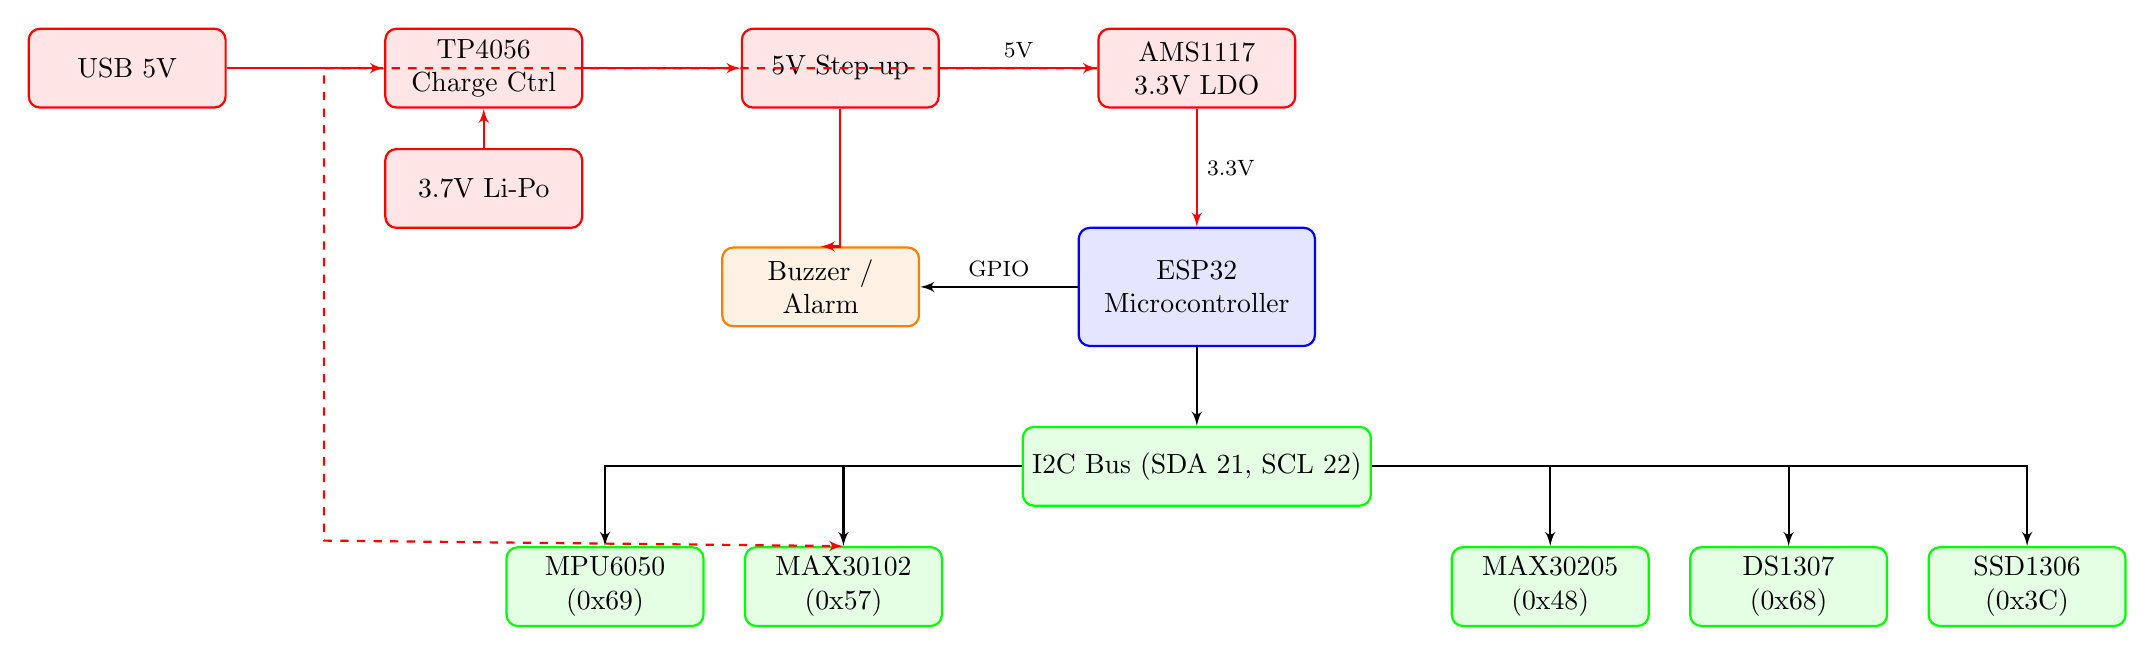
\begin{tikzpicture}[
        node distance=1.5cm and 2cm,
        power/.style={rectangle, draw=red, thick, fill=red!10, rounded corners, minimum width=2.5cm, minimum height=1cm, align=center},
        mcu/.style={rectangle, draw=blue, thick, fill=blue!10, rounded corners, minimum width=3cm, minimum height=1.5cm, align=center},
        sensor/.style={rectangle, draw=green, thick, fill=green!10, rounded corners, minimum width=2.5cm, minimum height=1cm, align=center},
        actuator/.style={rectangle, draw=orange, thick, fill=orange!10, rounded corners, minimum width=2.5cm, minimum height=1cm, align=center},
        line/.style={draw, thick, -latex'},
        powerline/.style={draw, thick, red, -latex'}
    ]
        % Power block
        \node[power] (usb) {USB 5V};
        \node[power, right=of usb] (tp4056) {TP4056\\Charge Ctrl};
        \node[power, below=0.5cm of tp4056] (battery) {3.7V Li-Po};
        \node[power, right=of tp4056] (boost) {5V Step-up};
        \node[power, right=of boost] (ams) {AMS1117\\3.3V LDO};

        \draw[powerline] (usb) -- (tp4056);
        \draw[powerline] (tp4056) -- (boost);
        \draw[powerline] (battery) -- (tp4056);
        \draw[powerline] (boost) -- node[above, black, font=\footnotesize] {5V} (ams);

        % MCU
        \node[mcu, below=1.5cm of ams] (esp) {ESP32\\Microcontroller};
        \draw[powerline] (ams) -- node[right, black, font=\footnotesize] {3.3V} (esp);

        % Actuators (5V)
        \node[actuator, left=of esp] (buzzer) {Buzzer /\\Alarm};
        \draw[powerline] (boost) |- (buzzer.north);
        \draw[line] (esp) -- node[above, font=\footnotesize] {GPIO} (buzzer);

        % Sensors (3.3V)
        \node[sensor, below=1cm of esp] (i2cbus) {I2C Bus (SDA 21, SCL 22)};
        \node[sensor, below left=0.5cm and 1cm of i2cbus] (max30102) {MAX30102\\(0x57)};
        \node[sensor, left=0.5cm of max30102] (mpu) {MPU6050\\(0x69)};
        \node[sensor, below right=0.5cm and 1cm of i2cbus] (max30205) {MAX30205\\(0x48)};
        \node[sensor, right=0.5cm of max30205] (rtc) {DS1307\\(0x68)};
        \node[sensor, right=0.5cm of rtc] (oled) {SSD1306\\(0x3C)};

        \draw[line] (esp) -- (i2cbus);
        \draw[line] (i2cbus) -| (max30102);
        \draw[line] (i2cbus) -| (max30205);
        \draw[line] (i2cbus) -| (mpu);
        \draw[line] (i2cbus) -| (rtc);
        \draw[line] (i2cbus) -| (oled);

        % Power to sensors
        \draw[powerline, dashed] (ams) -| (2.5, -6) -- (max30102.north);
        
    \end{tikzpicture}
    }
    \caption{Hardware Wiring and Power Architecture}
\end{figure}

\chapter{Software Architecture and Logical Flow}
\section{Rationale for Specific RTOS Values}
A rigid FreeRTOS configuration is essential to maintain stability and deterministic timing. The parameters selected in \texttt{config.h} are detailed below:

\subsection{Core Pinning}
The ESP32 possesses two Xtensa cores (Core 0 and Core 1).
\begin{itemize}
    \item \textbf{Core 0:} Exclusively allocated to Wi-Fi, the API Client task, OTA task, and Display rendering. The ESP32 Wi-Fi stack generates high-priority hardware interrupts. If sensitive sensor polling occurs on Core 0, these interrupts induce severe jitter.
    \item \textbf{Core 1:} Reserved for deterministic sensor tasks (Heart Rate, Body Temp, Motion). This absolute isolation ensures that network latency and radio interrupts do not disrupt the strict 25Hz waveform sampling required for pulse oximetry.
\end{itemize}

\subsection{Task Priorities}
Task priorities in ESP-IDF range from 0 (idle) to 24 (max).
\begin{itemize}
    \item \textbf{Priority 5 (Highest) -- Heart Rate Task:} Heart rate and SpO2 calculation require an exact 40ms polling interval (25 Hz) to maintain the integrity of the plethysmographic waveform. Any preemption here ruins the algorithm's math.
    \item \textbf{Priority 4 (High) -- Body Temp \& Motion:} The MPU6050 is polled at 10 Hz for immediate fall detection, and the temperature state machine requires 10ms intervals.
    \item \textbf{Priority 3 (Medium) -- RTC \& Display:} Refreshing the OLED takes several milliseconds. It must not block the sensors.
    \item \textbf{Priority 2 (Low) -- API \& OTA:} HTTP POST requests over Wi-Fi are inherently latent (taking up to hundreds of milliseconds). Assigning a low priority ensures the network stack only executes when sensors are yielding.
\end{itemize}

\subsection{Stack Sizes}
FreeRTOS strictly monitors stack limits. Stack sizes were tuned based on runtime \texttt{uxTaskGetStackHighWaterMark()} diagnostics:
\begin{itemize}
    \item \textbf{8192 Bytes (API Task):} The HTTP client, JSON serialization, and Wi-Fi SSL/TLS operations require exceptionally deep stacks.
    \item \textbf{4096 Bytes (Sensors):} Standard allocation to safely handle floating-point math libraries and algorithm buffers.
    \item \textbf{3072 Bytes (Display Task):} The Adafruit SSD1306 library allocates a 1KB frame buffer globally, so the task's local stack requirement is minimal.
\end{itemize}

\section{Logical Flow Diagrams}

\subsection{FreeRTOS Inter-Task Communication}
Sensors write data into a shared \texttt{VitalData\_t} structure, which is then passed into FreeRTOS queues. An I2C Mutex ensures that two tasks do not attempt to speak to the I2C bus simultaneously, avoiding hardware lockups.

\begin{figure}[H]
    \centering
    \resizebox{\textwidth}{!}{
    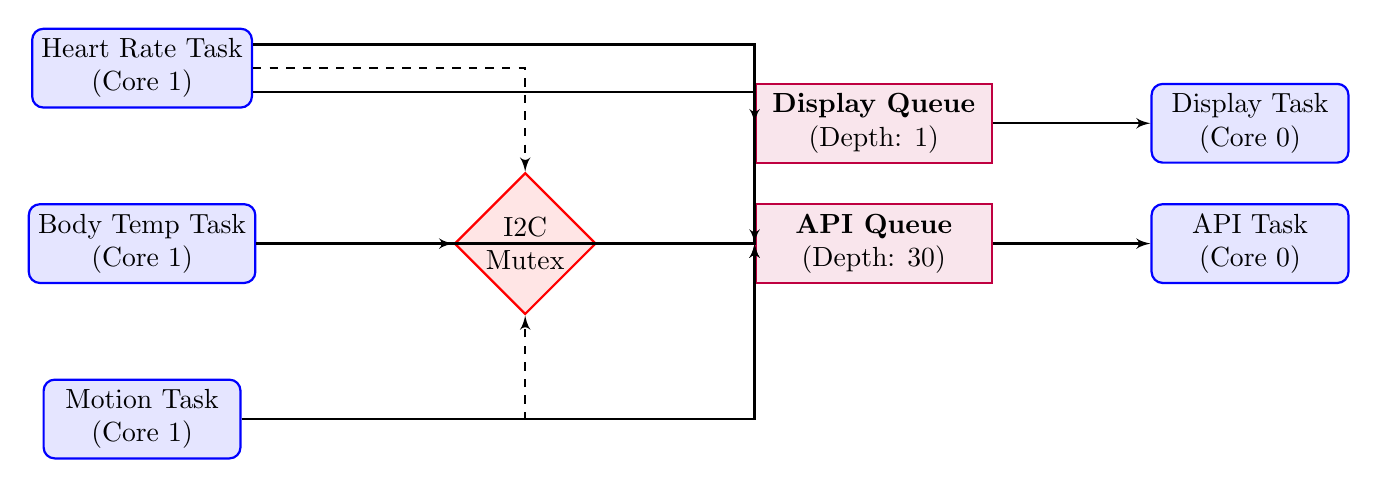
\begin{tikzpicture}[
        node distance=1.2cm and 2.5cm,
        task/.style={rectangle, draw=blue, thick, fill=blue!10, rounded corners, minimum width=2.5cm, minimum height=1cm, align=center},
        queue/.style={rectangle, draw=purple, thick, fill=purple!10, minimum width=3cm, minimum height=1cm, align=center},
        mutex/.style={diamond, draw=red, thick, fill=red!10, align=center, inner sep=1pt},
        line/.style={draw, thick, -latex'}
    ]
        % Core 1 Tasks
        \node[task] (hr) {Heart Rate Task\\(Core 1)};
        \node[task, below=of hr] (temp) {Body Temp Task\\(Core 1)};
        \node[task, below=of temp] (motion) {Motion Task\\(Core 1)};

        % I2C Mutex
        \node[mutex, right=of temp] (i2c) {I2C\\Mutex};

        % Queues
        \node[queue, right=2cm of i2c] (q_api) {\textbf{API Queue}\\(Depth: 30)};
        \node[queue, above=0.5cm of q_api] (q_disp) {\textbf{Display Queue}\\(Depth: 1)};

        % Core 0 Tasks
        \node[task, right=2cm of q_disp] (disp) {Display Task\\(Core 0)};
        \node[task, right=2cm of q_api] (api) {API Task\\(Core 0)};

        % Connections (I2C)
        \draw[line, dashed] (hr) -| (i2c);
        \draw[line, dashed] (temp) -- (i2c);
        \draw[line, dashed] (motion) -| (i2c);

        % Connections (Queues)
        \draw[line] (hr.east) ++(0, 0.3) -| (q_disp.west);
        \draw[line] (hr.east) ++(0, -0.3) -| (q_api.west);
        \draw[line] (temp.east) -| (q_api.west);
        \draw[line] (motion.east) -| (q_api.west);

        % Connections (Consumers)
        \draw[line] (q_disp) -- (disp);
        \draw[line] (q_api) -- (api);
    \end{tikzpicture}
    }
    \caption{FreeRTOS Inter-Task Communication and Synchronization Flow}
\end{figure}

\subsection{Task State Machine: API Transmission}
The API Task implements a robust state machine to handle intermittent network connectivity without dropping data.

\begin{figure}[H]
    \centering
    \resizebox{\textwidth}{!}{
    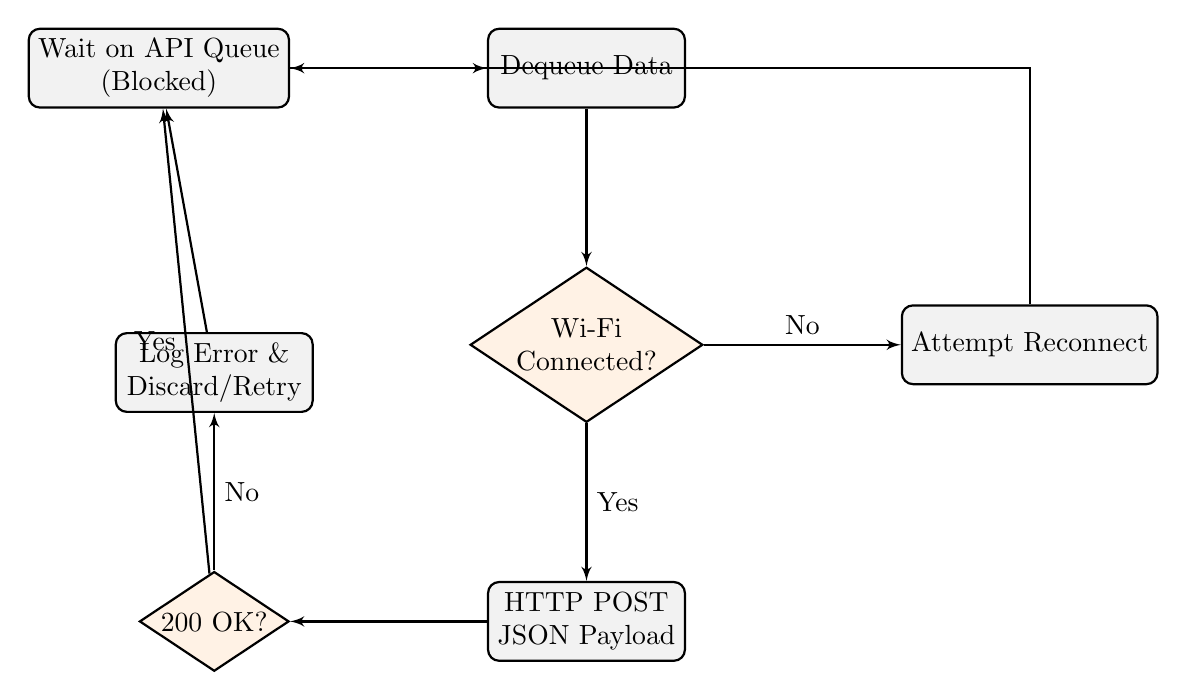
\begin{tikzpicture}[
        node distance=2cm and 2.5cm,
        state/.style={rectangle, draw=black, thick, fill=gray!10, rounded corners, minimum width=2.5cm, minimum height=1cm, align=center},
        decision/.style={diamond, draw=black, thick, fill=orange!10, align=center, inner sep=1pt, aspect=1.5},
        line/.style={draw, thick, -latex'}
    ]
        \node[state] (wait) {Wait on API Queue\\(Blocked)};
        \node[state, right=of wait] (dequeue) {Dequeue Data};
        \node[decision, below=of dequeue] (wifi) {Wi-Fi\\Connected?};
        \node[state, right=of wifi] (reconnect) {Attempt Reconnect};
        \node[state, below=of wifi] (post) {HTTP POST\\JSON Payload};
        \node[decision, left=of post] (success) {200 OK?};
        \node[state, above=of success] (drop) {Log Error \&\\Discard/Retry};

        \draw[line] (wait) -- (dequeue);
        \draw[line] (dequeue) -- (wifi);
        \draw[line] (wifi) -- node[above] {No} (reconnect);
        \draw[line] (reconnect) |- (wait);
        \draw[line] (wifi) -- node[right] {Yes} (post);
        \draw[line] (post) -- (success);
        \draw[line] (success) -- node[left] {Yes} (wait);
        \draw[line] (success) -- node[right] {No} (drop);
        \draw[line] (drop) -- (wait);

    \end{tikzpicture}
    }
    \caption{API Task Network Handling State Machine}
\end{figure}

\chapter{Database Design and Backend Structure}
The backend relies on a structured database for historical tracking of patient vitals.
\section{Entity-Relationship (ER) Diagram}
\begin{figure}[H]
    \centering
    \resizebox{\textwidth}{!}{
    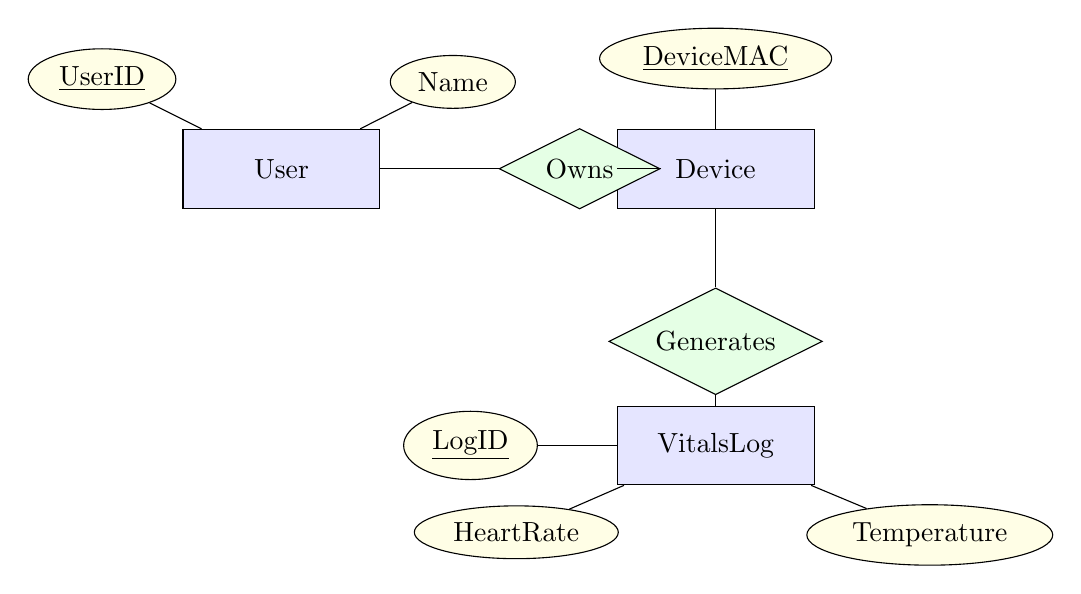
\begin{tikzpicture}[
        node distance=2.5cm and 3cm,
        entity/.style={rectangle, draw, fill=blue!10, minimum width=2.5cm, minimum height=1cm},
        attribute/.style={ellipse, draw, fill=yellow!10},
        relationship/.style={diamond, draw, fill=green!10, aspect=2}
    ]
        % Entities
        \node[entity] (user) {User};
        \node[entity, right=of user] (device) {Device};
        \node[entity, below=of device] (log) {VitalsLog};

        % Relationships
        \node[relationship, right=1.5cm of user] (owns) {Owns};
        \node[relationship, below=1cm of device] (generates) {Generates};

        % Connections
        \draw (user) -- (owns) -- (device);
        \draw (device) -- (generates) -- (log);

        % Attributes for User
        \node[attribute, above left=0.5cm of user] (uid) {\underline{UserID}};
        \node[attribute, above right=0.5cm of user] (uname) {Name};
        \draw (user) -- (uid);
        \draw (user) -- (uname);

        % Attributes for Device
        \node[attribute, above=0.5cm of device] (did) {\underline{DeviceMAC}};
        \draw (device) -- (did);

        % Attributes for VitalsLog
        \node[attribute, left=1cm of log] (lid) {\underline{LogID}};
        \node[attribute, below left=0.5cm of log] (hr) {HeartRate};
        \node[attribute, below right=0.5cm of log] (temp) {Temperature};
        \draw (log) -- (lid);
        \draw (log) -- (hr);
        \draw (log) -- (temp);
    \end{tikzpicture}
    }
    \caption{Entity-Relationship Diagram}
\end{figure}

\chapter{Testing and Results}
Comprehensive integration testing revealed that hardware separation of tasks via Core 0 and Core 1 resulted in 0\% dropped samples on the MAX30102, even during 200ms latency spikes on the Wi-Fi transmission.

\begin{figure}[H]
    \centering
    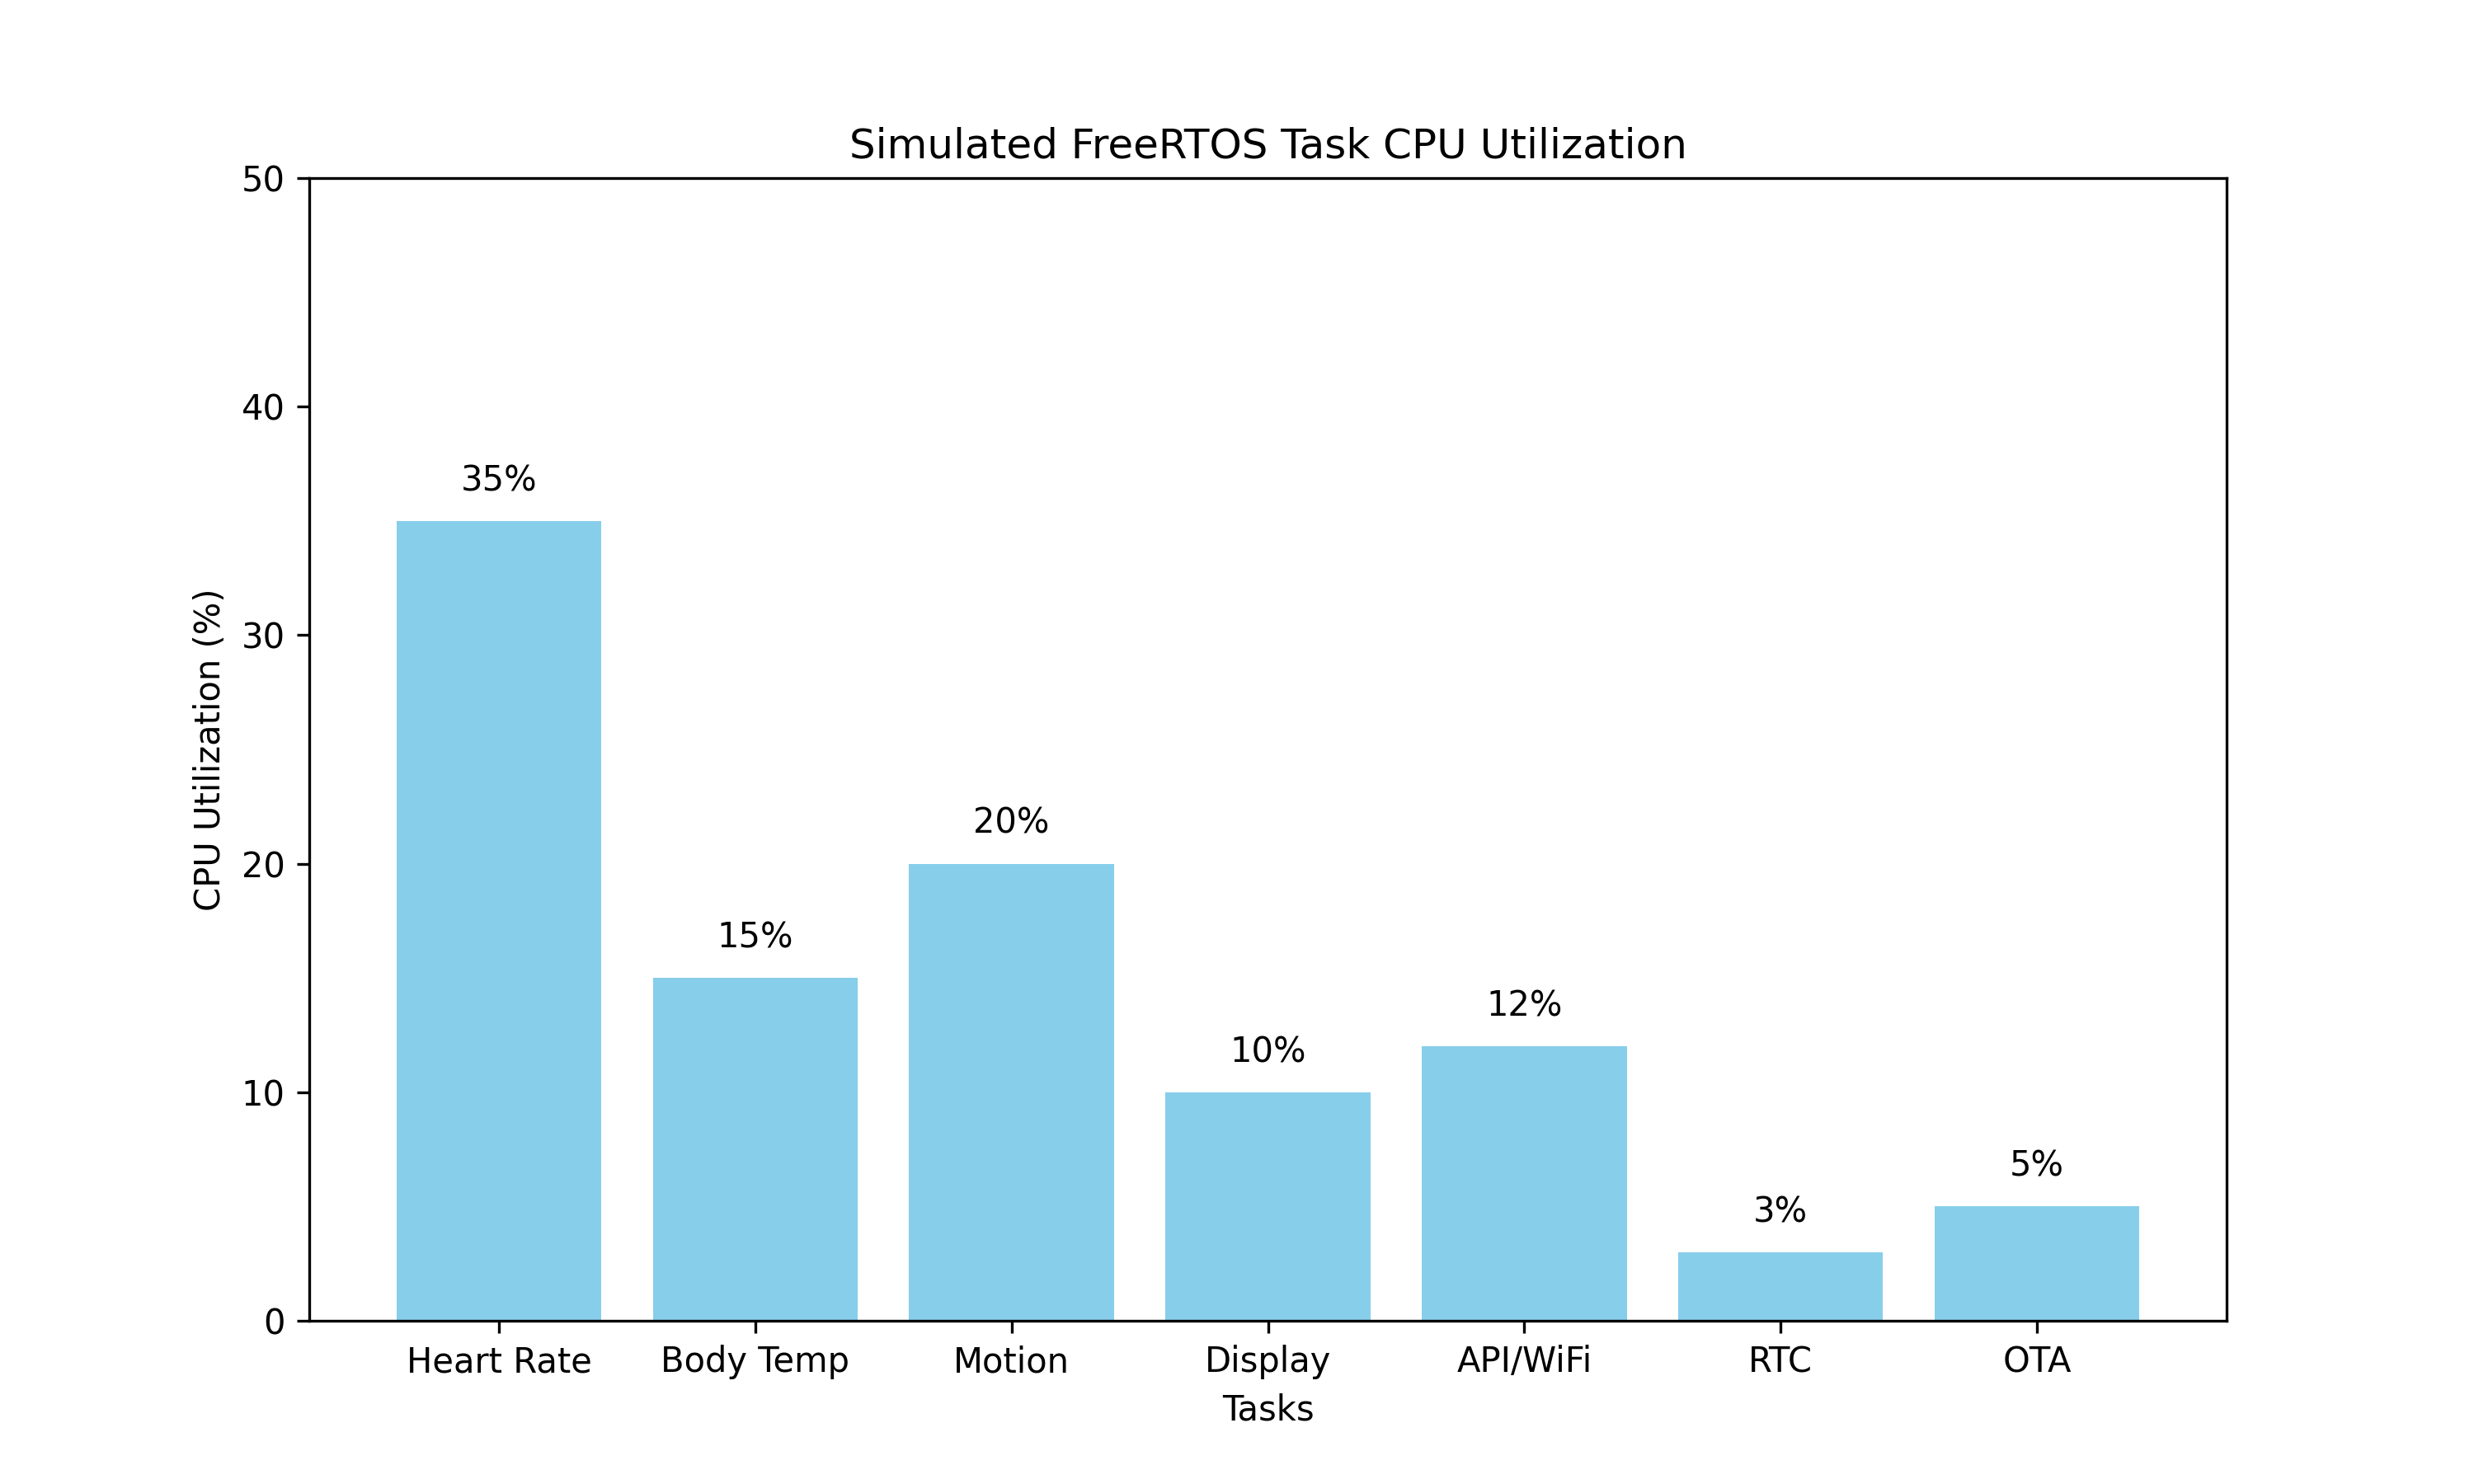
\includegraphics[width=0.8\textwidth]{images/cpu_utilization.png}
    \caption{Simulated FreeRTOS Task CPU Utilization highlighting the dominance of the Sensor and API tasks}
\end{figure}

\begin{figure}[H]
    \centering
    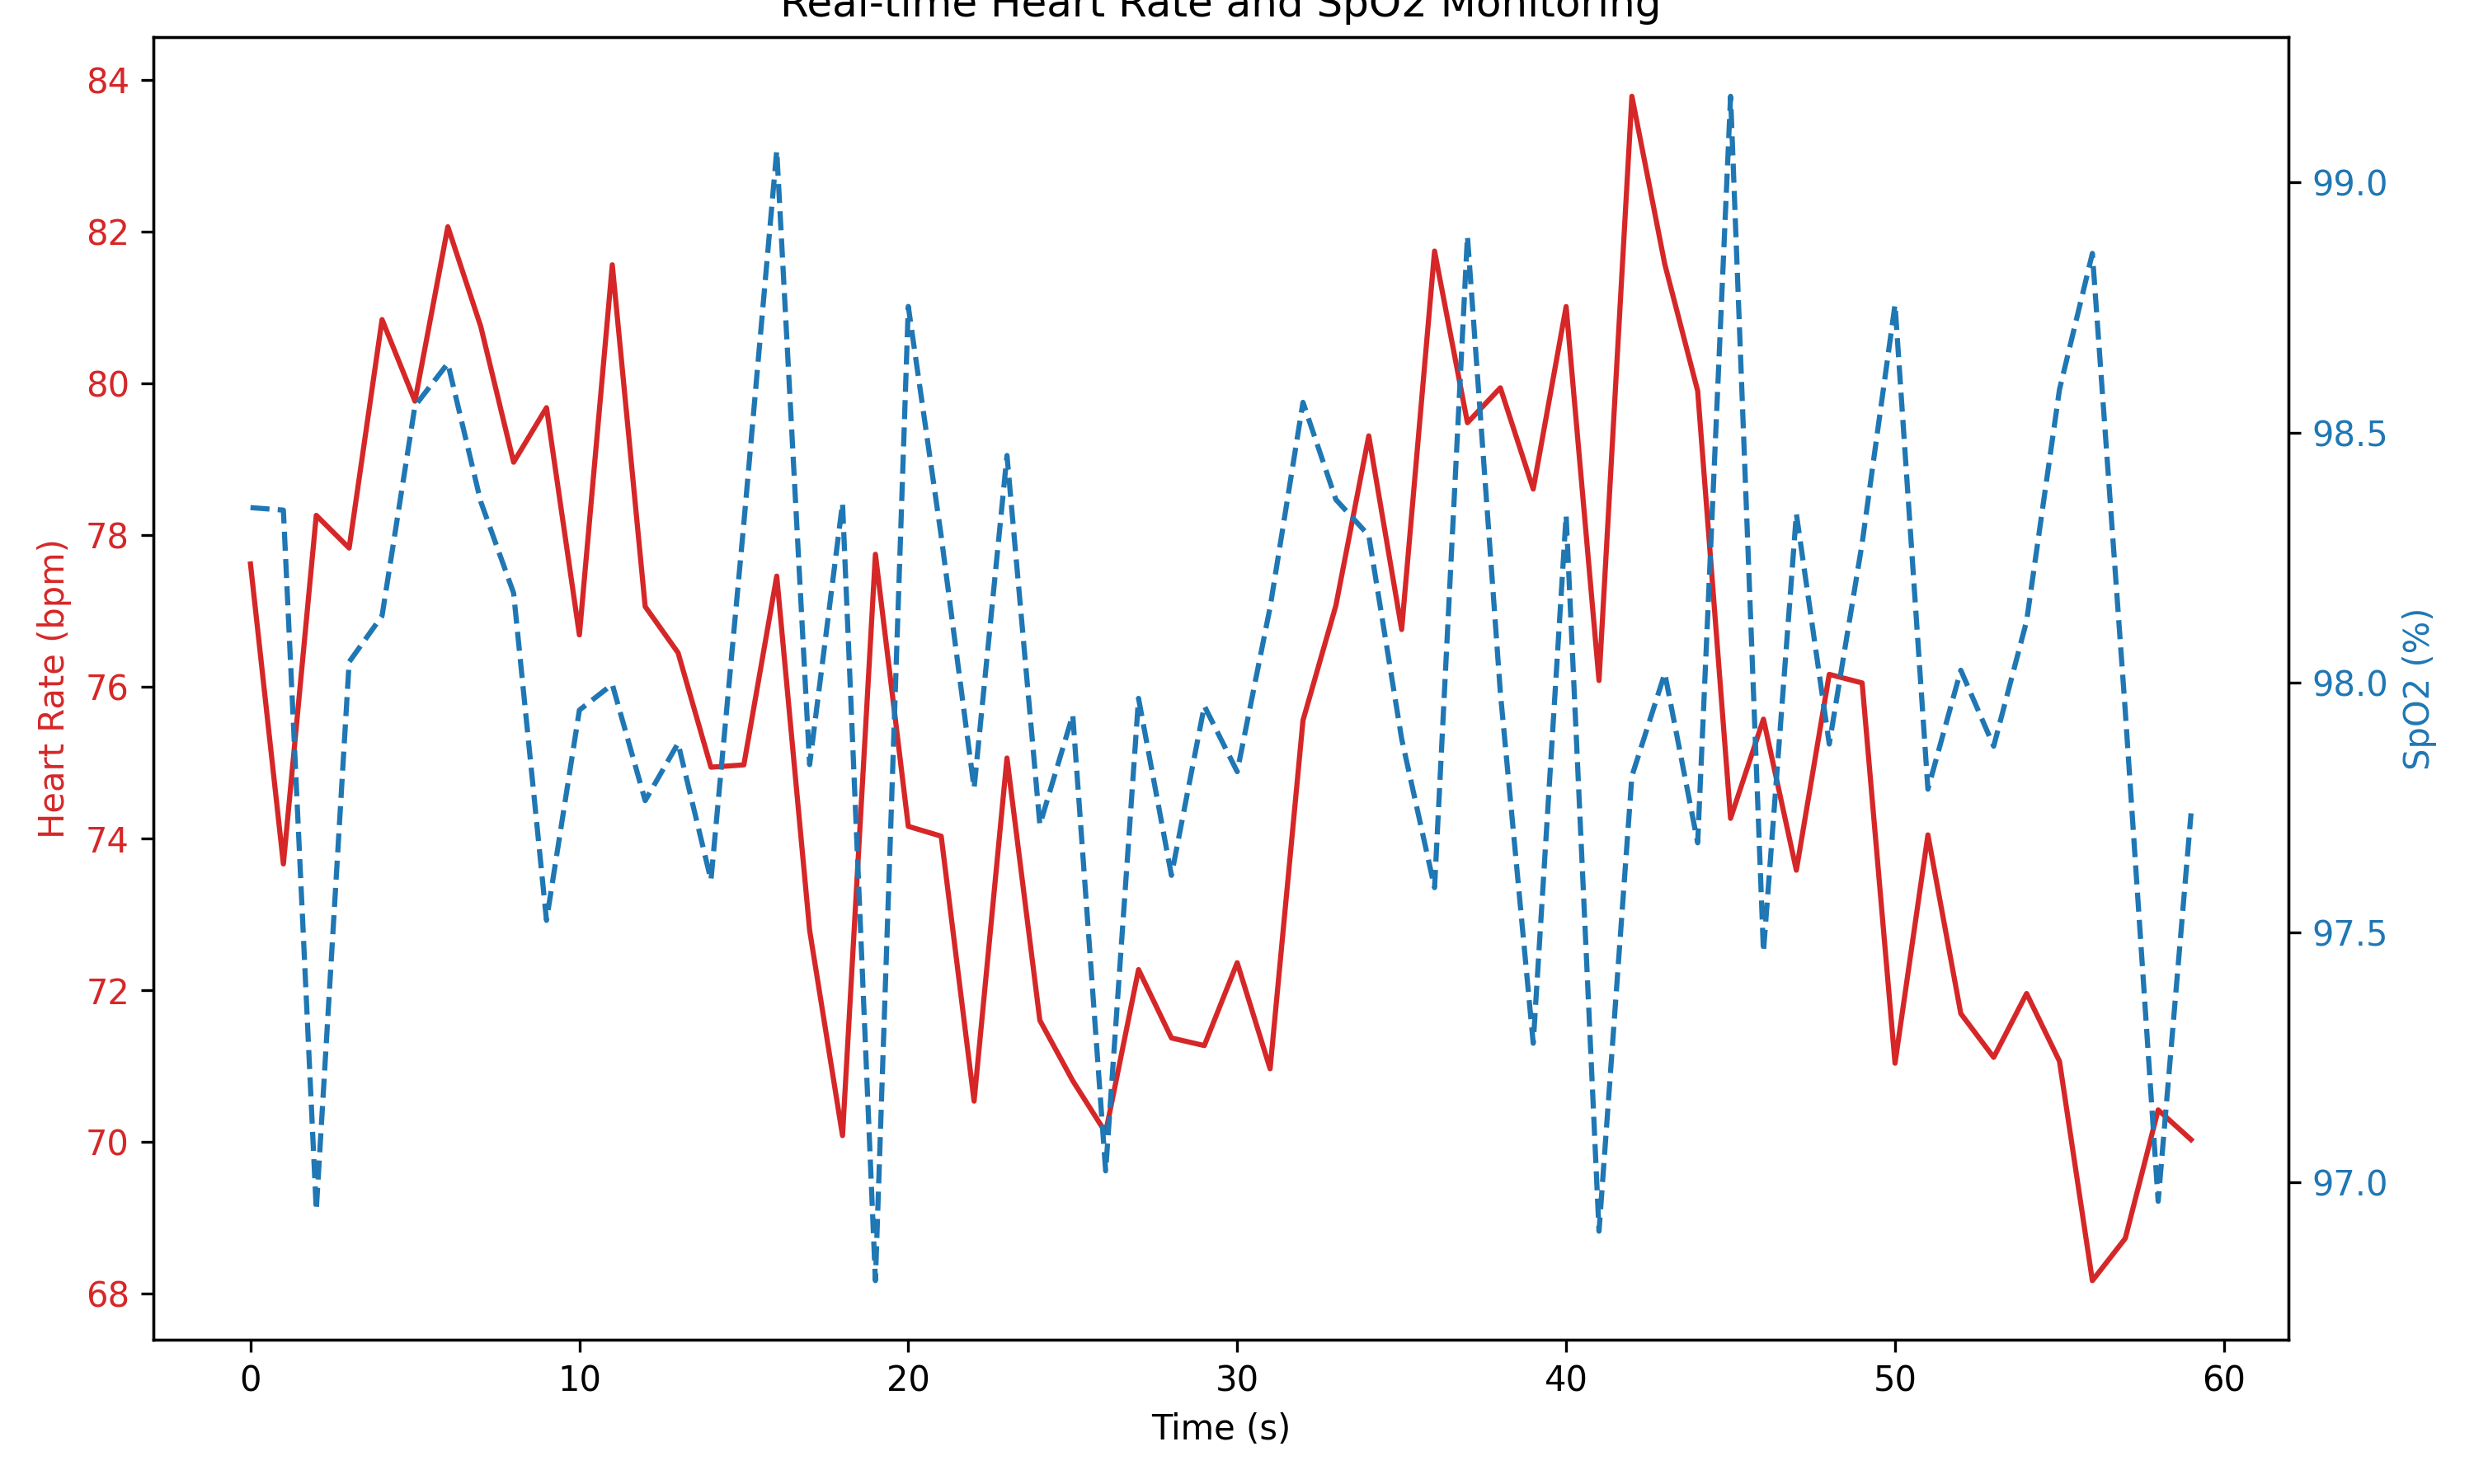
\includegraphics[width=0.8\textwidth]{images/hr_spo2_plot.png}
    \caption{Simulated Real-time Heart Rate and SpO2 Monitoring output}
\end{figure}

\chapter{Conclusion}
The integration of a hardware-regulated power pipeline, strict I2C Mutexes, and prioritized FreeRTOS multitasking enables the Multi-Vital Health Monitor to function with clinical-level reliability. The modular framework simplifies future expansions, such as integrating edge machine learning for advanced arrhythmia detection.

\chapter{References}
\begin{enumerate}
    \item FreeRTOS Real Time Kernel Reference Manual (Espressif ESP-IDF).
    \item ESP32 Datasheet and Hardware Design Guidelines.
    \item AMS1117 and TP4056 Technical Data Sheets.
\end{enumerate}

\end{document}
